The task of the removal station is to take a single sheet metal part from a stack of raw sheets and make it
available to the robot unit. This is a mechatronic system with several components, which all
have to function individually, but also together in combination. The mechatronic system is controlled by the \hyperref[acro:PLC]{PLC}.


\begin{figure}[h]
    \centering
    \begin{subfigure}{0.505\textwidth}
        \centering
        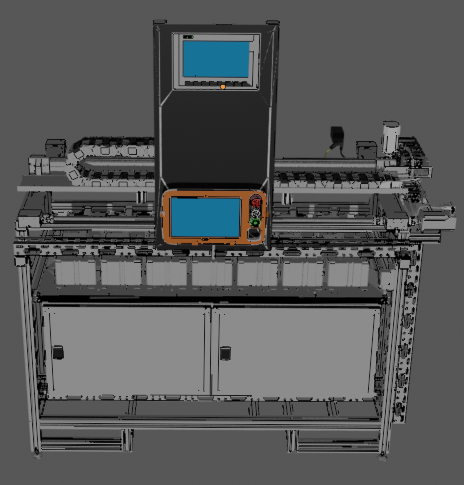
\includegraphics[width=\textwidth]{figures/unloading-station-front-blender.png} % Replace with your image file
        \caption{front-view}
        \label{fig:unloading-station-front}
    \end{subfigure}\hfill
    \begin{subfigure}{0.45\textwidth}
        \centering
        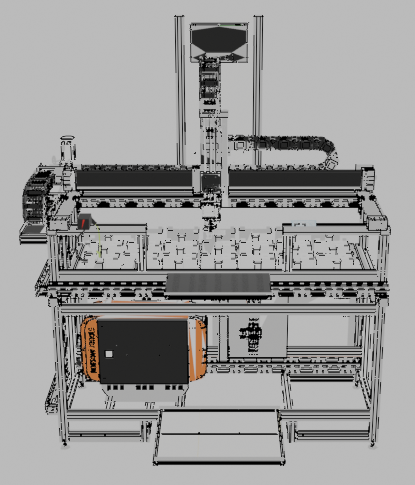
\includegraphics[width=\textwidth]{figures/unloading-station-back-blender.png} % Replace with your image file
        \caption{back-view}
        \label{fig:unloading-station-back}
    \end{subfigure}
    \caption{Unloading station in simulation}
    \label{fig:unloading-station}
\end{figure}

This unloading station is on top of a cabinet which houses the \hyperref[acro:PLC]{PLC} and controller of the handling robot.
